\documentclass[a4paper,12pt]{article}

\usepackage{url}
\usepackage{amsmath,amssymb}
\usepackage{setspace}
\usepackage{fontspec}             % for Thai unicode characters
\XeTeXlinebreaklocale "th"
\XeTeXlinebreakskip = 0pt plus 1pt
\usepackage[Latin,Thai]{ucharclasses}
\defaultfontfeatures{Mapping=tex-text} 
\setmainfont{TeX Gyre Termes}				% Free Times
\setsansfont{TeX Gyre Heros}				% Free Helvetica
\setmonofont{TeX Gyre Cursor}				% Free Courier
\newfontfamily{\thaifont}[Scale=MatchUppercase,Mapping=tex-text]{TH Sarabun New:script=thai}

\usepackage{listings}
\lstset{
basicstyle=\ttfamily,
numbers=left,
numberstyle=\small,
breaklines=true,
xleftmargin=.1\linewidth,
frame=single,
columns=fullflexible,
captionpos=b,
showstringspaces=false
}

\onehalfspacing

\setTransitionTo{Thai}{\thaifont}
\setTransitionFrom{Thai}{\normalfont}

\title{Fourier Transform}
\author{Wolfram MathWorld}
\date{}

\begin{document}
\maketitle
ข้อความข้างล่างนี้ตัดมาจาก \cite{WolframForier} ให้ทดลองเขียน source code ของ \LaTeX~เอง เพื่อสร้างเอกสารนี้ โครงของเอกสารคือไฟล์ Exercise.tex

\section{การอ้างถึง การแทรกรูป และการใส่เชิงอรรถ}
\begin{figure}[h]
\centering
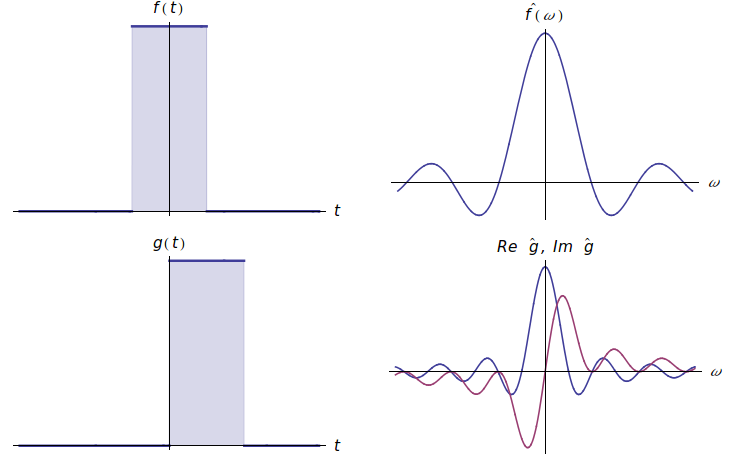
\includegraphics[width=.8\columnwidth]{ExercisesFig/Fourier_transform_of_rect_and_a_translation}
\caption{ตัวอย่างการแปลงฟูเรียร์}
\label{Fig:TransformExample}
\end{figure}
ภาพที่ \ref{Fig:TransformExample} นำมาจาก Wikipedia\footnote{``Fourier transform of rect and a translation'' by Slawekb - Created in Mathematica 9.0. Licensed under CC BY-SA 3.0 via Wikipedia - \url{https://en.wikipedia.org/wiki/File:Fourier_transform_of_rect_and_a_translation.png#/media/File:Fourier_transform_of_rect_and_a_translation.png}}

\section{การเขียนสมการ และการสร้างข้อย่อย}
ตัวอย่างข้างล่างนี้มีทั้งการเขียนคำสั่งคณิตศาสตร์แทรกระหว่างข้อความ และการกำหนดสภาพแวดล้อมคณิตศาสตร์ มีการใช้ cases ในการกำหนดค่าให้ฟังก์ชัน และการแทรกข้อความลงในสภาพแวดล้อมคณิตศาสตร์ ลองสังเกตดูว่าฟอนต์ที่ใช้ในสภาพแวดล้อมคณิตศาสตร์กับสภาพแวดล้อมข้อความปกตินั้นต่างกัน ผู้เขียนเอกสารพึงระวังเสมอเมื่อต้องการอ้างถึงตัวแปรต่าง ๆ

ส่วนเงื่อนไขด้านล่างใช้การสร้างข้อย่อยแบบมีเลขข้อ

A function $f(x)$ has a forward and inverse Fourier transform such that
\begin{equation}
 f(x)= \begin{cases}
 \int_{-\infty}^\infty e^(2 \pi ikx) \left[\int_{-\infty}^\infty f(x)e^{-2\pi ikx} dx \right]dk
     & \text{for } f(x) \text{ continuous at } x; \\
 \frac{1}{2}[f(x_+)+f(x_-)]
     & \text{for } f(x) \text{ discontinuous at } x, 	
 \end{cases} 
\end{equation}
provided that
\begin{enumerate}
\item $\int_{-\infty}^\infty|f(x)|dx$ exists.
\item There are a finite number of discontinuities.
\item The function has bounded variation. A sufficient weaker condition is fulfillment of the Lipschitz condition (Ramirez 1985, p. 29). The smoother a function (i.e., the larger the number of continuous derivatives), the more compact its Fourier transform.
\end{enumerate}

\section{การเขียนสมการ (เพิ่มเติม) และการสร้างตาราง}
\label{Sec:Table}
ตัวอย่างข้างล่างนี้เป็นการใช้สมการหลายบรรทัดและมีการจัดตำแหน่งให้ตรงกัน ในที่นี้จัดตำแหน่งของ $\equiv$ ให้ตรงกับ $=$ ในบรรทัดถัดมา นอกจากนี้ยังมีการใช้สัญลักษณ์พิเศษ $\star$ การใส่ bar เหนือตัวแปร ($\bar{f}$) รวมถึงฟอนต์พิเศษสำหรับ $\mathcal{F}, \mathbf{x}, \mathbf{k}$ และ $\mathbb{R}$ ด้วย สัญลักษณ์พิเศษเหล่านี้ต้องใช้ package amsmath และ amssymb ผู้ที่ต้องใช้สัญลักษณ์ทางคณิตศาสตร์เป็นประจำควรจดจำได้ว่าต้องใช้ฟอนต์แบบใดกับตัวแปรหรือสัญลักษณ์ที่ต้องการ

The ``autocorrelation width'' is
\begin{align}
w_a	&\equiv	\frac{\int_{-\infty}^\infty f \star \bar{f}dx}{[f \star \bar{f}]_0}	\\
	&=	\frac{\int_{-\infty}^\infty f dx \int_{-\infty}^\infty \bar{f}dx}{\int_{-\infty}^\infty f \bar{f} dx},	
\end{align}
where $f \star g$ denotes the cross-correlation of $f$ and $g$ and $\bar{f}$ is the complex conjugate.

Any operation on $f(x)$ which leaves its area unchanged leaves $F(0)$ unchanged, since
\begin{equation}
 \int_{-\infty}^\infty f(x) dx = \mathcal{F}_x[f(x)](0)=F(0). 	
\end{equation}
The following table summarized some common Fourier transform pairs.

\begin{tabular}{|l|l|l|}
\hline
function	& $f(x)$	& $F(k)=\mathcal{F}_x[f(x)](k)$ \\
\hline
Fourier transform--1
    & $1$
    & $\delta(k)$ \\
Fourier transform--cosine
    & $\cos(2\pi k_0x)$
    & $\frac{1}{2}[\delta(k-k_0)+\delta(k+k_0)]$ \\
Fourier transform--delta function
    & $\delta(x-x_0)$
    & $e^{-2\pi ikx_0}$ \\
Fourier transform--exponential function
    & $e^{-2\pi k_0|x|}$
    & $\frac{1}{\pi}\frac{k_0}{k^2+k_0^2}$ \\
Fourier transform--Gaussian
    & $e^{-ax^2}$
    & $\sqrt{\frac{\pi}{a}}e^{-\pi^2k^2/a}$ \\
Fourier transform--Heaviside step function
    & $H(x)$
    & $\frac{1}{2} \left[ \delta(k)-\frac{i}{\pi k} \right]$ \\
Fourier transform--inverse function
    & $-PV \frac{1}{\pi x}$
    & $i[1-2H(-k)]$ \\
Fourier transform--Lorentzian function
	& $\frac{1}{\pi}\frac{\frac{1}{2\Gamma}}{(x-x_0)^2+\left(\frac{1}{2}\Gamma \right)^2}$
	& $e^{-2\pi ikx_0-\Gamma \pi|k|}$ \\
Fourier transform--ramp function
	& $R(x)$
	& $\pi i \delta'(2\pi k) - \frac{1}{4\pi^2k^2}$ \\
Fourier transform--sine
	& $\sin(2\pi k_0x)$
	& $\frac{1}{2} i[\delta(k+k_0)-\delta(k-k_0)]$ \\
\hline
\end{tabular}
In two dimensions, the Fourier transform becomes
\begin{align}
F(x,y)	&=	\int_{-\infty}^\infty \int_{-\infty}^\infty f(k_x,k_y)e^{-2\pi i(k_x x + k_y y)} dk_x dk_y	\\
f(k_x,k_y)	&=	\int_{-\infty}^\infty \int_{-\infty}^\infty F(x,y)e^{2\pi i(k_x x + k_y y)} dx dy.	
\end{align}

การสร้างปีกกาใต้ข้อความข้างล่างนี้ใช้คำสั่ง
\begin{lstlisting}[numbers=none]
\underbrace{textabove}_{textbelow}
\end{lstlisting}

Similarly, the $n$-dimensional Fourier transform can be defined for $\mathbf{k}, \mathbf{x} \in \mathbb{R}^n$ by
\begin{align}
F(\mathbf{x})	&=	\underbrace{\int_{-\infty}^\infty \dots \int_{-\infty}^\infty}_n f(\mathbf{k})e^{-2\pi i \mathbf{k} \cdot \mathbf{x}}d^n \mathbf{k}	\\
f(\mathbf{k})	&=	\underbrace{\int_{-\infty}^\infty \dots \int_{-\infty}^\infty}_n F(\mathbf{x})e^{2\pi i \mathbf{k}\cdot \mathbf{x}}d^n \mathbf{x}.
\end{align}

\section{ข้อสังเกตอื่นๆ}
Caption ใต้ภาพยังเป็น Figure อยู่ ซึ่งเกิดจากคลาส article ที่ใช้นั้นกำหนดไว้เป็นภาษาอังกฤษ หากต้องการปรับให้เป็นภาษาไทย สามารถตั้งให้เป็นคำที่ต้องการเองได้โดยใช้คำสัง renewcommand เช่น หากสั่ง \lstinline|\renewcommand{\figurename}{Fig.}| Caption ของรูปจะเปลี่ยนจากค่าเริ่มต้นเติม (Figure) ไปเป็น Fig. เป็นต้น

ในคลาส chula นั้นมีคำสั่งกำหนดคำให้แล้วทั้งภาษาไทยและภาษาอังกฤษ ซึ่งสามารถเลือกใช้ได้โดยกำหนด option ของคลาสเป็น thaithesis หรือ engthesis

ตารางในข้อ \ref{Sec:Table} นั้นไม่มีชื่อตารางกำกับ และยังยาวเกินกว่าขอบเขตของข้อความที่กำหนด

\bibliographystyle{plain}
\bibliography{Exercise}
\end{document}